% Copyright (C) 2014-2020 by Thomas Auzinger <thomas@auzinger.name>

\documentclass[draft,final]{vutinfth} % Remove option 'final' to obtain debug information.

\usepackage{url}

% Load packages to allow in- and output of non-ASCII characters.
\usepackage{lmodern}        % Use an extension of the original Computer Modern font to minimize the use of bitmapped letters.
\usepackage[T1]{fontenc}    % Determines font encoding of the output. Font packages have to be included before this line.
\usepackage[utf8]{inputenc} % Determines encoding of the input. All input files have to use UTF8 encoding.

% Extended LaTeX functionality is enables by including packages with \usepackage{...}.
\usepackage{amsmath}    % Extended typesetting of mathematical expression.
\usepackage{amssymb}    % Provides a multitude of mathematical symbols.
\usepackage{mathtools}  % Further extensions of mathematical typesetting.
\usepackage{microtype}  % Small-scale typographic enhancements.
\usepackage[inline]{enumitem} % User control over the layout of lists (itemize, enumerate, description).
\usepackage{multirow}   % Allows table elements to span several rows.
\usepackage{booktabs}   % Improves the typesettings of tables.
\usepackage{subcaption} % Allows the use of subfigures and enables their referencing.
\usepackage[ruled,linesnumbered,algochapter]{algorithm2e} % Enables the writing of pseudo code.
\usepackage[usenames,dvipsnames,table]{xcolor} % Allows the definition and use of colors. This package has to be included before tikz.
\usepackage{nag}       % Issues warnings when best practices in writing LaTeX documents are violated.
\usepackage{todonotes} % Provides tooltip-like todo notes.
\usepackage{hyperref}  % Enables cross linking in the electronic document version. This package has to be included second to last.
\usepackage[acronym,toc]{glossaries} % Enables the generation of glossaries and lists fo acronyms. This package has to be included last.

% Define convenience functions to use the author name and the thesis title in the PDF document properties.
\newcommand{\authorname}{Jacob Palecek} % The author name without titles.
\newcommand{\thesistitle}{Improving Serverless Edge Computing for Network Bound Workloads} % The title of the thesis. The English version should be used, if it exists.

% Set PDF document properties
\hypersetup{
    pdfpagelayout   = TwoPageRight,           % How the document is shown in PDF viewers (optional).
    linkbordercolor = {Melon},                % The color of the borders of boxes around crosslinks (optional).
    pdfauthor       = {\authorname},          % The author's name in the document properties (optional).
    pdftitle        = {\thesistitle},         % The document's title in the document properties (optional).
    pdfsubject      = {Subject},              % The document's subject in the document properties (optional).
    pdfkeywords     = {a, list, of, keywords} % The document's keywords in the document properties (optional).
}

\setpnumwidth{2.5em}        % Avoid overfull hboxes in the table of contents (see memoir manual).
\setsecnumdepth{subsection} % Enumerate subsections.

\nonzeroparskip             % Create space between paragraphs (optional).
\setlength{\parindent}{0pt} % Remove paragraph identation (optional).

\makeindex      % Use an optional index.
\makeglossaries % Use an optional glossary.
%\glstocfalse   % Remove the glossaries from the table of contents.

% Set persons with 4 arguments:
%  {title before name}{name}{title after name}{gender}
%  where both titles are optional (i.e. can be given as empty brackets {}).
\setauthor{}{\authorname}{BSc.}{male}
\setadvisor{Univ.Prof. Dr.}{Schahram Dustdar}{}{male}

% For bachelor and master theses:
\setfirstassistant{Dr.}{Thomas Rausch}{}{male}
% \setsecondassistant{Pretitle}{Forename Surname}{Posttitle}{male}
% \setthirdassistant{Pretitle}{Forename Surname}{Posttitle}{male}

% For dissertations:
% \setfirstreviewer{Pretitle}{Forename Surname}{Posttitle}{male}
% \setsecondreviewer{Pretitle}{Forename Surname}{Posttitle}{male}

% For dissertations at the PhD School and optionally for dissertations:
% \setsecondadvisor{Pretitle}{Forename Surname}{Posttitle}{male} % Comment to remove.

% Required data.
\setregnumber{01526624}
\setdate{01}{08}{2020} % Set date with 3 arguments: {day}{month}{year}.
\settitle{\thesistitle}{Improving Serverless Edge Computing for Network Bound Workloads} % Sets English and German version of the title (both can be English or German). If your title contains commas, enclose it with additional curvy brackets (i.e., {{your title}}) or define it as a macro as done with \thesistitle.
% \setsubtitle{Optional Subtitle of the Thesis}{Optionaler Untertitel der Arbeit} 
% Sets English and German version of the subtitle (both can be English or German).

% Select the thesis type: bachelor / master / doctor / phd-school.
% Bachelor:
% \setthesis{bachelor}
%
% Master:
\setthesis{master}
\setmasterdegree{dipl.} % dipl. / rer.nat. / rer.soc.oec. / master
%
% Doctor:
%\setthesis{doctor}
%\setdoctordegree{rer.soc.oec.}% rer.nat. / techn. / rer.soc.oec.
%
% Doctor at the PhD School
%\setthesis{phd-school} % Deactivate non-English title pages (see below)

% For bachelor and master:
\setcurriculum{Software Engineering and Internet Computing}{Software Engineering und Internet Computing} % Sets the English and German name of the curriculum.

% For dissertations at the PhD School:
\setfirstreviewerdata{Affiliation, Country}
\setsecondreviewerdata{Affiliation, Country}


\begin{document}

\frontmatter % Switches to roman numbering.
% The structure of the thesis has to conform to the guidelines at
%  https://informatics.tuwien.ac.at/study-services

\addtitlepage{naustrian} % German title page (not for dissertations at the PhD School).
\addtitlepage{english} % English title page.
\addstatementpage

\begin{danksagung*}
\todo{Ihr Text hier.}
\end{danksagung*}

\begin{acknowledgements*}
\todo{Enter your text here.}
\end{acknowledgements*}

\begin{kurzfassung}
\todo{Ihr Text hier.}
\end{kurzfassung}

\begin{abstract}
\todo{Enter your text here.}
\end{abstract}

% Select the language of the thesis, e.g., english or naustrian.
\selectlanguage{english}

% Add a table of contents (toc).
\tableofcontents % Starred version, i.e., \tableofcontents*, removes the self-entry.

% Switch to arabic numbering and start the enumeration of chapters in the table of content.
\mainmatter
\newacronym{fet}{FET}{Function Execution Time}
\newacronym{csv}{CSV}{Comma separated values}
\newacronym{cpu}{CPU}{Central Processing Unit}
\newacronym{ram}{RAM}{Random Access Memory}
\newacronym{gpu}{GPU}{Grahpics Processing Unit}
\newacronym{wan}{WAN}{Wide Area Network}
\newacronym{ran}{RAN}{Radio Access Network}
\newacronym{rtt}{RTT}{Round Trip Time}
\newacronym{trt}{TRT}{Total Response Time}
\newacronym{rps}{rps}{requests per second}
\newacronym{sla}{SLA}{Service Level Agreement}
\newacronym{qos}{QoS}{Quality of Service}
\newacronym{jsq}{JSQ}{Join-the-Shortest-Queue}
\newacronym{jiq}{JIQ}{Join-the-Idle-Queue}
\newacronym{jfsq}{JFSQ}{Join-the-Fastest-of-the-Shortest-Queue}
\newacronym{jfiq}{JFIQ}{Join-the-Fastest-of-the-Idle-Queue}
\newacronym{iot}{IoT}{Internet of Things}
\newacronym{iiot}{IIoT}{Industrial Internet of Things}
\newacronym{ai}{AI}{Artificial Intelligence}
\newacronym{mec}{MEC}{Mobile Edge Computing}
\newacronym{hpa}{HPA}{Horizontal Pod Autoscaler}
\newacronym{faas}{FaaS}{Function as a Service}
\newacronym{paas}{PaaS}{Platform as a Service}
\newacronym{tdp}{TDP}{Thermal Design Power}
\newacronym{kpi}{KPI}{Key Performance Indicator}
\newacronym{iaas}{IaaS}{Infrastructure as a Service}

\chapter{Introduction}
\section{Motivation}
\section{Problem Statement}
\section{Research Questions}

\begin{enumerate}
        \item How can current scaling and placement techniques for load balancers be changed, such that the overall performance of the serverless edge computing system improves?\\\\
    Serverless (edge) computing frameworks typically already possess a mechanism for scaling and placing services. It is also typical for load balancers to be treated as "just another service", and thus identically to functions\cite{openfaas}.
    Conceptually this is not surprising since load balancers, like functions, can be scaled to handle more requests than a single instance could.
    Serverless frameworks do not, however, consider the special role load balancers play in the performance of the system in edge computing scenarios.
    To improve the performance, particularly of network bound workloads, the scaling and placement techniques used for load balancers will likely need to be changed. As a result, we need to answer the question how the used techniques in that area have to be adapted in order to realize the aspired performance improvements, while still considering the potential side effects this has on the overall system.

        \item How much of a performance improvement can be gained from optimizing the scaling, placement and decisions of load balancers in serverless edge computing systems?\\\\
    When investigating what changes could be made to increase system responsiveness in serverless edge computing, particularly for network bound workloads, load balancing stands out as an area that is likely to yield significant improvements. Current serverless computing systems do not possess the scaling, placement and load balancing mechanisms required to process requests efficiently in an edge computing scenario. Their implementation is based on the assumption of relative homogeneity in compute power and network structure one typically finds in cloud computing systems. Even serverless computing frameworks specifically built or adapted for the edge do not necessarily take the heterogeneity of edge computing environments into account when it comes to load balancing\cite{skippy}.
    This leaves the question of whether or not adapting serverless edge computing frameworks in regard to the scaling and placement of load balancers, as well as their load balancing decision mechanism, results in performance improvements, and if so, how large they likely are.
    
        \item How do edge optimized scaling and placement techniques for load balancers, including the load balancing techniques themselves, affect the overall system behavior and characteristics in regard to their key performance metrics?\\\\
    In a serverless computing framework there usually exists an interplay between a number of different components, such as the scaler and the scheduler\cite{openfaas}\cite{kubernetes}. 
    When parts of the system are now changed, in this case, the way in which load balancers behave, as well as how they are scaled and placed, this change is potentially liable to affect the rest of the system. Some of these effects would of course be intended, such as better end to end latency, but there could also be additional, potentially unwanted effects. It is thus important how exactly such changes affect the system, and what implications that has. These changes are measured in the form of key performance indicators.
\end{enumerate}
\section{Approach}
% 1 page
Our objective with this thesis is to improve serverless computing for network bound workloads. 
The improvements we aim for are focused primarily on reducing response time, which has already been identified as an issue \cite{skippy}, but are likely also translatable to efficiency gains, depending on what the implementation goals of the specific system in question are.


Our initial evaluation identified load balancing as the primary factor holding back the performance of serverless edge computing for network bound workloads, and we thus aim to make improvements in this area.
As our preliminary testing showed, the minimum requirements to make meaningful improvements in this area are that load balancers need to be distributed across the network  instead of being centralized, and that they need to make more sophisticated load balancing decisions.
To this end our goal is two-fold.
First, we want to present a method for scaling and scheduling load balancers in such a way that they are close enough to both clients and function replicas in the network to enable requests to take an efficient path between the two.
Second, we will propose a load balancing scheme that makes load balancing decisions, which take into account the network distance of clients and function replicas, as well as the replicas' performance.


To evaluate different approaches for load balancer placement and load balancing decisions we use and extend a state of the art serverless computing simulator, and ground those simulations on real data where possible by building upon existing research\cite{philipp-da}, and conducting additional experiments to inform the simulator's functioning.
This way our methodology allows us to explore scenarios beyond those feasible for live-hardware experimentation, while making sure results are as representative as possible by using performance profiles generated via experiments with actual hardware \cite{thomas-thesis}.
Apart from simulations in the context of serverless computing, we perform separate simulations and experiments in related areas, deepening the understanding and showing the relation between the challenges of serverless edge computing and the broader context.

We further explore more than just end user performance metrics, also showing how the different components present in modern serverless solutions are influenced and themselves influence methods for load balancing and placing load balancer replicas.
Through this we gain an understanding of, outline, and propose a potential solution for the engineering problems that need to be solved in order to improve serverless edge computing in practice.
\section{Structure}
Chapter 2 provides relevant background information for the technological environment this work is embedded in. In particular it outlines the concept of serverless computing, serverless edge computing, as well as describing the concepts of load balancing and service placement.
Chapter 3 explores the related work, highlighting which other works are most directly related to this one, and describing how this thesis differs from them.
Chapter 4 describes our proposed approach. After a brief overview of the general concept, it gives insight into our view of the problem domain, followed by detailed explanations of our approach and the rationale that led to it.
Chapter 5 describes the methodologies we used when evaluating our approach, explaining the serverless function as well as its relevant components, and how it informs its simulation with data from experiments on actual hardware.
Chapter 6 contains the evaluations of our approach, detailing both experiment setups and results.
These results are then discussed in chapter 7, where their implications for serverless edge, but also the limitations of our approach are explained.
Lastly, chapter 8 concludes this thesis and gives and outlook on future work.



\chapter{Background}
\section{Serverless Computing}
% got 4 pages
This section aims to give an overview of serverless computing.
Readers who are well-versed within the matter can feel free to skip this introduction, and reference it only when needed
\subsection{What serverless computing is}
Serverless computing emerged as a new computing paradigm in the context of cloud computing, which delegates infrastructure provisioning and configuration to the cloud provider to alleviate software developers from that burden.
\gls{faas} is one of the most prominent types of serverless computing products on offer.
It allows developers to specify serverless functions, which are then deployed and scaled by the cloud provider.
It is a way in which software developers architect, develop, and deploy applications that is dramatically different from more traditional approaches.
In traditional approaches, such as microservice architectures, an application is partitioned into small components which can be scaled and deployed independently of each other.
Although microservice architectures often rely on the \gls{iaas} or \gls{paas} solutions cloud providers offer, and thus abstract away the underlying infrastructure to a certain degree, developers still need to handle most scaling and application specific \gls{qos} requirements themselves.

From a developer's perspective, serverless computing is a further increase in abstraction \cite{jonasCloudProgrammingSimplified2019}.
It can be seen as the next step in an evolution away from monolithic software applications.
Where microservices and containerized deployments first partitioned a large application into several smaller applications, serverless computing continues this trend of division into smaller components, since in serverless computing applications are partitioned into individual \textit{functions}, which each perform a single action\cite{khandelwalTaureauDeconstructingServerless2020}.

\begin{figure}
    \centering
    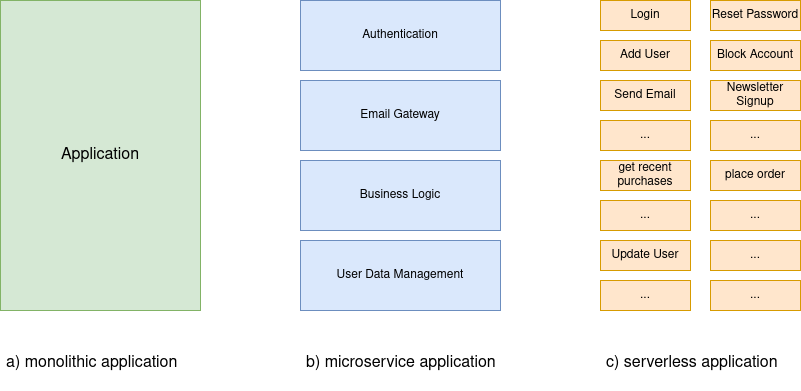
\includegraphics[width=\columnwidth]{graphics/diagrams/monolith_micro_serverless.png}
    \caption{Conceptual overview of different application architecture paradigms}
    \label{fig:mono_micro_serverless}
\end{figure}

Figure \ref{fig:mono_micro_serverless} shows this transition towards smaller partitioning of application code, leading to a higher and higher level of abstraction.
Just like microservices enabled application developers to scale different aspects of an application independently, thus enabling elasticity, serverless computing takes this even further allowing individual functions of the application to be scaled separately from each other\cite{jonasCloudProgrammingSimplified2019}.

Overall serverless affords application developers a number of advantages:
\begin{itemize}
    \item \textbf{Arbitrary elasticity:} As mentioned, serverless applications can scale their components on an extremely fine-grained level\cite{khandelwalTaureauDeconstructingServerless2020}
    \item \textbf{Abstracted infrastructure:} Where previously developers needed to be at least somewhat cognizant of the deployment of their application or its microservices, serverless enables this task to be fully delegated to the cloud provider. Developers don't necessarily need any knowledge of cloud infrastructure\cite{jonasCloudProgrammingSimplified2019}.
    \item \textbf{Precise Billing:} While in traditional cloud computing environments resources are leased for a set amount of time, irrespective of their actual usage\cite{khandelwalTaureauDeconstructingServerless2020}, serverless features a billing model where only the actual execution time and memory footprint of a function is billed down to millisecond precision\cite{jonasCloudProgrammingSimplified2019}. This allows for better resource utilization and potentially reduced costs from a customer's perspective\cite{khandelwalTaureauDeconstructingServerless2020}.
\end{itemize}

While these advantages of serverless computing over more traditional approaches are compelling, there are also idiosyncrasies of serverless computing that can, depending on the application, be problematic.
These include the need for statelessness, meaning that serverless functions have no inherent capacity to store data and would instead need to fetch it from yet another service\cite{khandelwalTaureauDeconstructingServerless2020}, or potential performance inconsistencies from cold-starts.
A cold-start, which means that the specific function code isn't running and has to be started before the request can be serviced, can occur because a serverless function wasn't executed for a certain time\cite{wangPeekingCurtainsServerless2018}.

\subsection{The architecture of serverless systems}
Architecturally, serverless systems are closely related to event based systems.
Their general concept is also very similar, since an event (i.e. a request) first arrives at the system in a form of queue, where a dispatcher or load balancer decides what action needs to be taken based on the event, and forwards it to the service (i.e. function), which ultimately processes it\cite{castroServerDeadLong2019}.

Prominent cloud based serverless platforms such as AWS Lambda\cite{aws-lambda} and Azure Functions\cite{azure-functions} are, however, proprietary and their precise architecture and inner workings are thus unknown to the public.
How these systems behave is a topic of ongoing research\cite{wangPeekingCurtainsServerless2018}, but since our research requires precise knowledge of implementation details, we choose to use open source serverless frameworks as a reference architecture of serverless systems.
These systems include Apache OpenWhisk\cite{openwhisk}, Kubeless\cite{kubeless}, and OpenFaaS\cite{openfaas}.
Since OpenFaaS has already been adapted for serverless edge computing by Rausch et al.\cite{rauschServerlessPlatformEdge}, we choose to use this open source serverless framework as the stand-in for serverless computing frameworks in general.

Architecturally, OpenFaaS is structured very similarly to the generic serverless architecture described by Castro et al.\cite{castroServerDeadLong2019}.
It too has a centralized entry-point, the Gateway, which sends requests to specific function replicas or alternatively to a queue (used for asynchronous processing and dealing with requests to functions that aren't currently running).
Each Gateway is thus effectively a load balancer for the serverless functions.
Figure \ref{fig:openfaas-gateway-diagram} shows a diagram of the architecture, as it is found in their official documentation\cite{openfaas-gateway}.

From a technical perspective, a key aspect of OpenFaaS' implementation is that it uses containers to host functions.
Containers provide an abstraction over Linux based operating systems, allowing for easier management of software dependencies, more closely controlled execution environments, and stronger application isolation.
Each function is packaged into such a container, which is an almost fully self-contained and portable artifact, that allows executing the developers' code on any machine with a compatible container runtime.
Functionally they behave similar to virtual machines, although they start up much faster, and aren't actually running individual kernels, which is why they do not provide the same level of security isolation true virtual machines do.
This choice allows functions to execute reliably, no matter the environment, and also makes it entirely agnostic to the programming language developers wish to use.
Since using containers entails their management over a cluster of multiple nodes, a task which is extremely complex, OpenFaaS\cite{openfaas} as well as other serverless frameworks build on Kubernetes\cite{kubernetes}, the de-facto industry standard container orchestration and management platform.
Building upon Kubernetes to deal with container management is a common choice among open source serverless frameworks, a choice which OpenWhisk and Kubeless make as well\cite{mohantyEvaluationOpenSource2018}.

OpenFaaS delegates a large number of tasks to the underlying Kubernetes cluster, including name resolution, request routing, which includes load balancing, and potentially scaling.
For this work, the delegation of load balancing decisions is especially important, since it implies that OpenFaaS uses whichever load balancing algorithm Kubernetes uses internally to distribute requests among function replicas.
Scaling, which determines how many instances of a serverless functions are running at any given time, can work via different mechanisms in OpenFaaS.
Depending how OpenFaaS is configured, it can either use Kubernetes' integrated \gls{hpa}\cite{kubernetes-hpa} or its own internal mechanism, which optionally allows for user customized scaling behavior\cite{openfaas-autoscaling}.
Since this work also aims to explore the impact a change in scaling and scheduling load balancers can have on the behavior of these scaling systems in general, we will now briefly describe the default scaling behavior of both \gls{hpa} and OpenFaaS' own scaler.

\subsubsection{Kubernets \gls{hpa}}
In Kubernetes scaling is typically based on either CPU or memory utilization, although in principle it can be extended with user-provided custom metrics\cite{kubernetes-hpa}.
For a given deployment, which in the context of serverless computing would be a function, a target resource value is defined.
An example would be a target average CPU utilization of 50\% for a type of function.
At that point, Kubernetes decides in a linear fashion what the desired number of replicas is.

Let $\mathbf{r_{\text{current}}}$ be the number of current replicas, $\mathbf{m_{\text{current}}}$ the current value of the metric in question and $\mathbf{m_{\text{target}}}$ the target value of the metric.
Then the target replica count is

\[ r_{\text{target}} = \left \lceil r_{\text{current}} \times \frac{m_{\text{current}}}{m_{\text{target}}} \right \rceil\]

To prevent inconsistent behavior such as replica counts oscillating Kubernetes also allows certain limiters to be set, such as minimum and maximum scales, rate of change for adding or removing replicas, and cool-downs which give the system time to stabilize before new scaling decisions are considered\cite{kubernetes-hpa}.

\subsubsection{OpenFaaS scaling}
The OpenFaaS integrated scaling mechanism is comprised of different parameters.
First a minimum and maximum scale must be set, which determine the effect of the scaling factor.
In this custom scaling variant system parameters, such as the request rate of a given function, are continuously evaluated.
Once a configured condition is met the system is notified that a given function needs to scale up or down.
The aforementioned scaling factor, which is a percentage value between 0 and 100, is then used to determine how many replicas should be started or stopped\cite{openfaas-autoscaling}.
Each scaling iteration adds or removes a number of replicas relative to the maximum scale allowed, and the scaling factor determines the size of that share.
If, for example, the maximum number of replicas is 50, and the scaling factor is 10\%, then at each scaling operation 5 replicas will be added or removed.

Which exact conditions trigger a scale up or scale down event within OpenFaaS is extremely configurable, and allows for customization based on an individual function's requirements.
By default, OpenFaaS triggers a scale-up event if the rate of rise of a function's invocation frequency exceeds a threshold over a period of time.




\section{Serverless Edge Computing}
% give a brief introduction to edge computing, just what it is + the obligatory graphic.
% what is serverless edge computing then?
% why don't current systems work well on the edge?
% give example of what it is necessary for -> edge intelligence, the bunch of applications that I've gathered, etc.
% about 2 pages should do just nicely

Serverless edge computing is an extension of existing serverless computing frameworks to the edge of the network.
It is an area of ongoing research, and aims to both further the adoption of edge computing and enable new use cases\cite{nasticServerlessRealTimeData2017}.

\subsection{Edge Computing}
Edge Computing has been proposed as a new computing paradigm to address a number of limitations and shortcomings of centralized cloud computing.
Edge Computing means that computations are not performed in a singe centralized location like a data center, but close to where the computations are needed or requested from, i.e. the edge of the network\cite{shiPromiseEdgeComputing2016}.

\begin{figure}
    \centering
    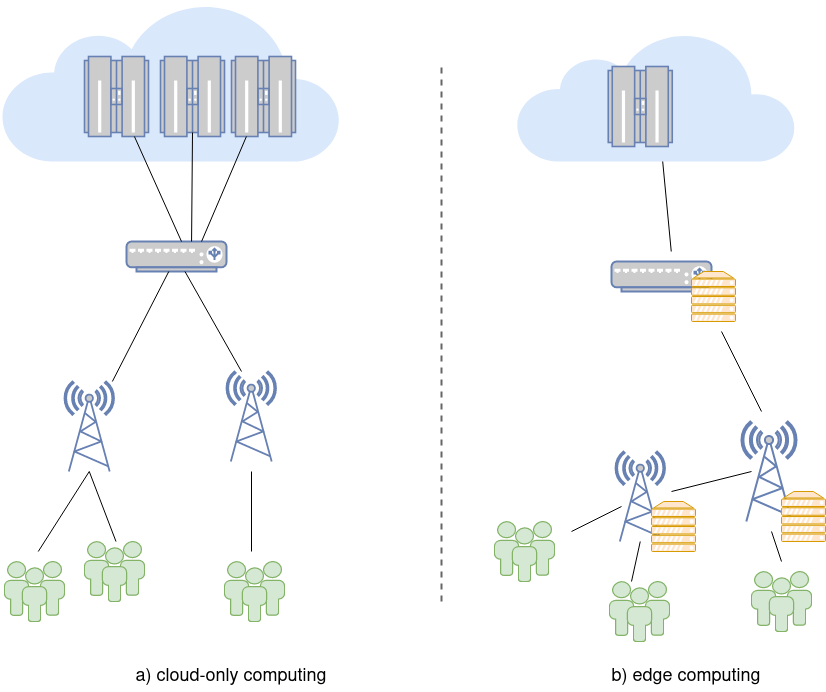
\includegraphics[width=12cm]{graphics/diagrams/edge_computing_example.png}
    \caption{An example of how in b) edge computing there are nodes interspersed throughout the network and close to clients, while in a) cloud computing all computation is centralized.}
    \label{fig:edge_comp_example}
\end{figure}

Edge computing enables a number of structural benefits that allow for the creation of new types of use-case and application.
Most notably, edge computing enables low latency, high bandwidth, computation offloading.
This can be used to improve application responsiveness, perform computations not possible on low-powered devices, or conserve energy on mobile devices by offloading complex computations to nearby edge nodes\cite{abbasMobileEdgeComputing2018b}.
Edge computing can also been seen as a way to transparently improve cloud computing, reducing the overall traffic in the network and making existing cloud applications more responsive by moving them closer to the user\cite{satyanarayananEmergenceEdgeComputing2017}.
Figure \ref{fig:edge_comp_example} shows the difference between edge and cloud computing in a simplified way.
In the example edge computing features computational nodes on \gls{ran}-towers, and thus much closer to the users.


This computing paradigm does, however, pose a challenge to existing frameworks and application architectures.
Given that computation resources are spread  farther throughout the network, the network infrastructure itself in edge computing is much more diverse\cite{shiEdgeComputingVisionChallenges2016}, potentially consisting of anything from the unreliable mobile network connection of a user's device to high bandwidth fiber networks between cloud data centers.
From both a hardware and software perspective, the computation hardware itself is more heterogeneous as well, requiring specific optimization mechanism to use resources in the most efficient way possible\cite{abbasMobileEdgeComputing2018b}.

\subsection{Serverless at the Edge}
Since serverless computing offers an abstraction layer on top of the actual infrastructure \cite{jonasCloudProgrammingSimplified2019}, and a key challenge of edge computing is that edge applications, at least up to now, have to be specifically crafted for their deployment scenario by developers\cite{shiPromiseEdgeComputing2016}.

With future \gls{ai} applications being dependent on edge computing to deliver their benefits to users via augmented reality, and smart city infrastructure\cite{rauschEdgeIntelligenceConvergence2019}, serverless offers an attractive abstraction layer to develop such \gls{ai} applications in an edge-native way.
Building on serverless as an abstraction layer for the application, the idea is that it will be able to jointly provide the benefits afforded by edge computing and serverless computing at the same time.
Functions are supposed to be deployed to nodes close to the users that rely on these functions, be scaled automatically, and routed efficiently, without any manual intervention from developers.

Achieving such a computing infrastructure would enable a host of new types of application, such as wearable cognitive assistance\cite{haWearableCognitiveAssistance2014}\cite{rauschPlatformSmartCityScale2021}, offloading \gls{ai} inference tasks from devices with low compute capability\cite{liEdgeAIOnDemand2020}, and analyzing video feeds in real time to improve public safety\cite{zhangEdgeVideoAnalytics2019}, for example to ensure face masks are worn where mandated\cite{wangWearMaskFastInbrowser2021}.

Open source serverless frameworks have been evaluated in terms of their performance in edge-scenarios, but in their current, unmodified state they lack the full set of capabilities needed to provide all the benefits edge computing offers\cite{paladeEvaluationOpenSource2019}.
While some of these serverless frameworks have been adapted to address the challenges posed by the edge computing environment, or to be better tailored to workloads related to \gls{ai}\cite{rauschServerlessPlatformEdge}, more of which will be discussed in the next chapter, overall there remain a lot of challenges for the universal practical application of serverless edge computing\cite{aslanpourServerlessEdgeComputing2021}.
Optimizing the performance of network bound workloads, for example, is one such challenge\cite{skippy}, and the one this thesis aims to address.




\section{Load Balancing}
\section{Service Placement}
% Target: 20ish pages total; 13 pages of text, 7 pages of images
\chapter{Approach}
In this chapter we describe our chosen approach for improving the performance of network bound workloads in serverless edge computing environments. We start by explaining our considerations when developing our approach in the context of a serverless edge computing system, and showing in what way our solution changes the system. From there we go into detail about how the load balancing mechanism of our solution works, how it is different from the currently employed methods, and how the choices made in regard to the load balancing method inform other parts of the proposed approach.
Lastly we go into our approach to scaling and scheduling load balancers among the nodes present in the serverless edge computing system. We make use of osmotic scaling and scheduling, a method previously outlined in existing literature. Using this idea of osmotic scaling and scheduling, we provide a concrete implementation of such an approach for placing and deciding on the number of load balancers in the system. The implementation is designed with current state of the art systems such as Kubernetes as the basis, and can thus be used as a reference implementation for use outside of a simulation context. The approach also addresses the challenges of edge computing environments that make current approaches, developed with the cloud in mind, unsuitable. Specifically our approach addresses issues of location awareness, device and network heterogeneity, and dynamically changing workload conditions.
% Target: 2ish pages \w graphics
\section{Concept}
% Note: mention that in our context load balancing and entry-gateway are sort of equivalent. Show their relation a bit
% Note: Mention that our approach uses the method of using real-life experiments to inform simulation

To understand the approach we first take a step back to view the boarder technical context the solution addresses and is built around.
As previously outlined, our solution aims to improve the performance of network bound workloads.
In the context of serverless edge computing systems network bound workloads are characterized by the network being the main or a significant contributing factor to the overall response time.
\begin{figure}
    \centering
    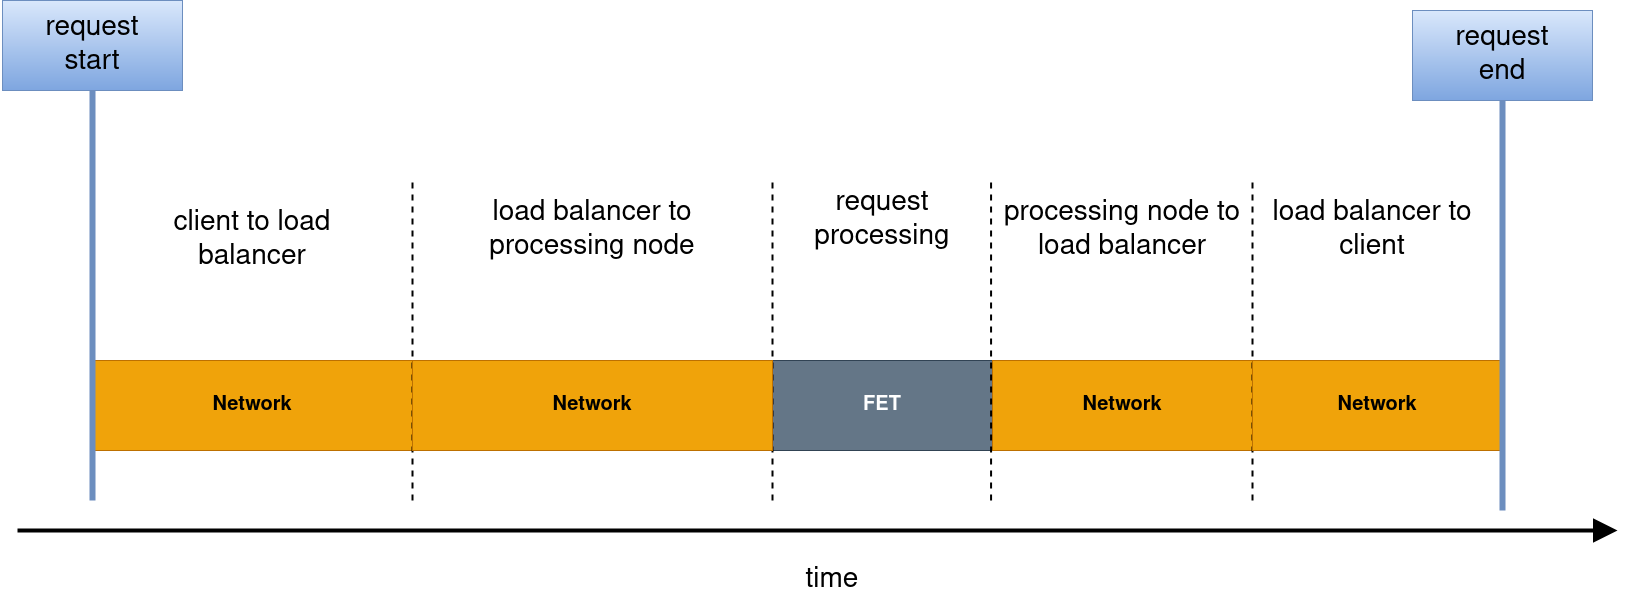
\includegraphics[width=14cm]{graphics/diagrams/request_overview.png}
    \caption{A generic view of the different parts that make up the total request processing time from the perspective of our approach}
    \label{fig:request_net_fet_overview}
\end{figure}
In Figure \ref{fig:request_net_fet_overview} we can see the different processing steps we consider for a request.
A network bound workload in this sense is one where the time taken up by the network portion of handling the request is proportionally speaking significantly larger than the portion taken by the \gls{fet}.
This is typically the case because either the request contains a lot of data that needs to be transported, or because the \gls{fet} is very short.

The primary way by which our approach improves the response times of network bound workloads is thus by reducing the amount of time spent on the network transfer portion of handling a client request.
While optimizing \glspl{fet} is not the primary objective of our approach, at least from a systems design perspective, it still has the potential to additionally reduce \glspl{fet} compared to current methods.
We consider the structure and makeup of the serverless computing system to be a given factor. As a result our approach aims to reduce network times not by changing the network makeup itself, but by utilizing the existing resources as effectively as possible. From a network-optimization perspective this means that each request should take an optimal path from  the client to the node where the request is ultimately processed. 

\begin{figure}
    \centering
    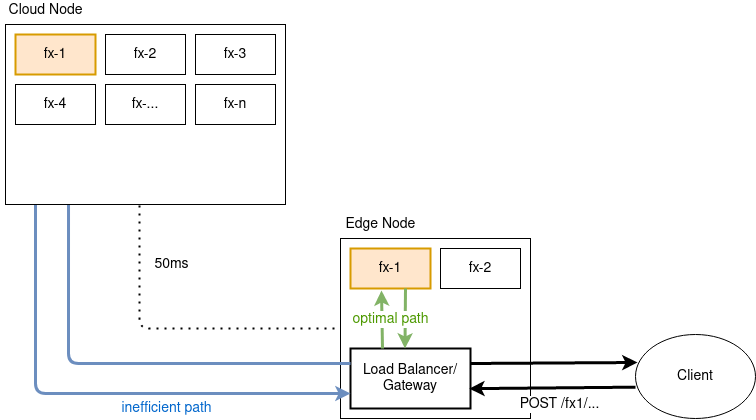
\includegraphics[width=12cm]{graphics/diagrams/efficient_path_example.png}
    \caption{Example diagram showing efficient and inefficient request routing based on network delay. "fx-1" through "fx-2" denote different types of function, and the dotted line denotes a network link between the cloud and edge node with a latency of 50ms}
    \label{fig:efficient_path}
\end{figure}

As can be understood quite intuitively in Figure \ref{fig:efficient_path}, round robin load balancing will in many cases lead to clearly suboptimal choices in terms of incurred network delay. The figure also shows the three key components we consider when trying to make network location based decisions: The client, the load balancer, and the node. Because our approach solely considers application level load balancers, since serverless platforms typically require these for their advanced routing decisions, any given request takes a path from the client to the load balancer, then to the selected upstream node, and back the same way.

Subsequently we want to incur the minimal amount of delay possible from both the hop between the client and load balancer, as well as between the load balancer and upstream node. Our proposed approach handles these two kinds of hops separately, at least for the most part. Since the scope of this work does not include optimizing the location of the serverless function instances themselves, this means we can improve performance through the following methods:
\begin{enumerate}
    \item \textbf{Intelligent load balancing decisions:} load balancers should choose upstream nodes that are both close in the network, and have \glspl{fet} short enough as not to negate the performance won through network proximity
    \item \textbf{Effective placement of load balancers:} the scheduler of the serverless system should place load balancers at locations in the network where they are in close proximity to clients and serverless function instances requested by these clients
    \item \textbf{Efficient scaling of load balancers:} the amount of load balancers should be high enough to provide the needed performance improvement, but not so high that the resources consumed by the load balancers diminish or even negate that effect
\end{enumerate}
In our approach the first method is provided by the load balancer itself. It is continuously updated with information where function instances, typically also referred to as \textit{replicas}, are located. Based on this and other information gathered by the load balancer, it tries to make decisions that lead to faster overall request responsiveness by selecting upstreams that are close and provide fast \glspl{fet}.

The other two methods are handled by the osmotic joint scaling and scheduling component of our approach. While the different methods of improvement are split between these two components of our proposed solution, this does not mean that they are completely separate from each other. Naturally the scheduling and scaling decisions will influence the way in which the placed load balancers work, while these in-turn affect the data gathered for and available to the scaling and scheduling component. The specifics of these two components will be discussed in the next two sections. 

It is also important to note that a significant amount of the approaches' implementation details are not chosen arbitrarily, but are rather the result of continuous cycle of experimentation and evaluation. While not detailed in the approach, the evaluation, result, and discussion chapters of this thesis include some of these experiments, in particular those that give additional insight into the problem domain and yielded results useful beyond informing this specific approach.
% Target: 8 pages with figures
\section{Load Balancers}
In this section we describe the role the load balancer plays in the context of our approach, how it is related to the underlying serverless platform, and the details of how it is implemented.

\subsection{ Definition \& Role In a Typical Serverless Framework}
First, we want to discuss what component exactly we mean by \textit{load balancer}, and how it functions in the context of a serverless framework. While our approach is not tied to any specific serverless framework, implementation, or technology, we developed it with their general concepts and functioning in mind. Because of this we feel that is helpful and informative to explain the components of our system in the context of an actual implementation, since this helps understand the abstract role these components play. In addition this is helpful for anyone who might want to integrate our approach into a production ready serverless edge computing platform.

As previously mentioned there are a number of different serverless frameworks, some free, some open source, some commercial, and some that fall in-between \cite{aws-lambda}\cite{azure-functions}\cite{openfaas-gateway}\cite{kubeless}\cite{openwhisk}.
We choose OpenFaaS\cite{openfaas}
as our reference implementation of a serverless framework because it is open source, allowing us detailed understanding of its inner workings, because it has been extended, for edge computing, and because it builds on and makes use of well established technologies in the same way other serverless frameworks do\cite{kubeless}\cite{openwhisk}, thus making it representative for the space.


\begin{figure}
    \centering
    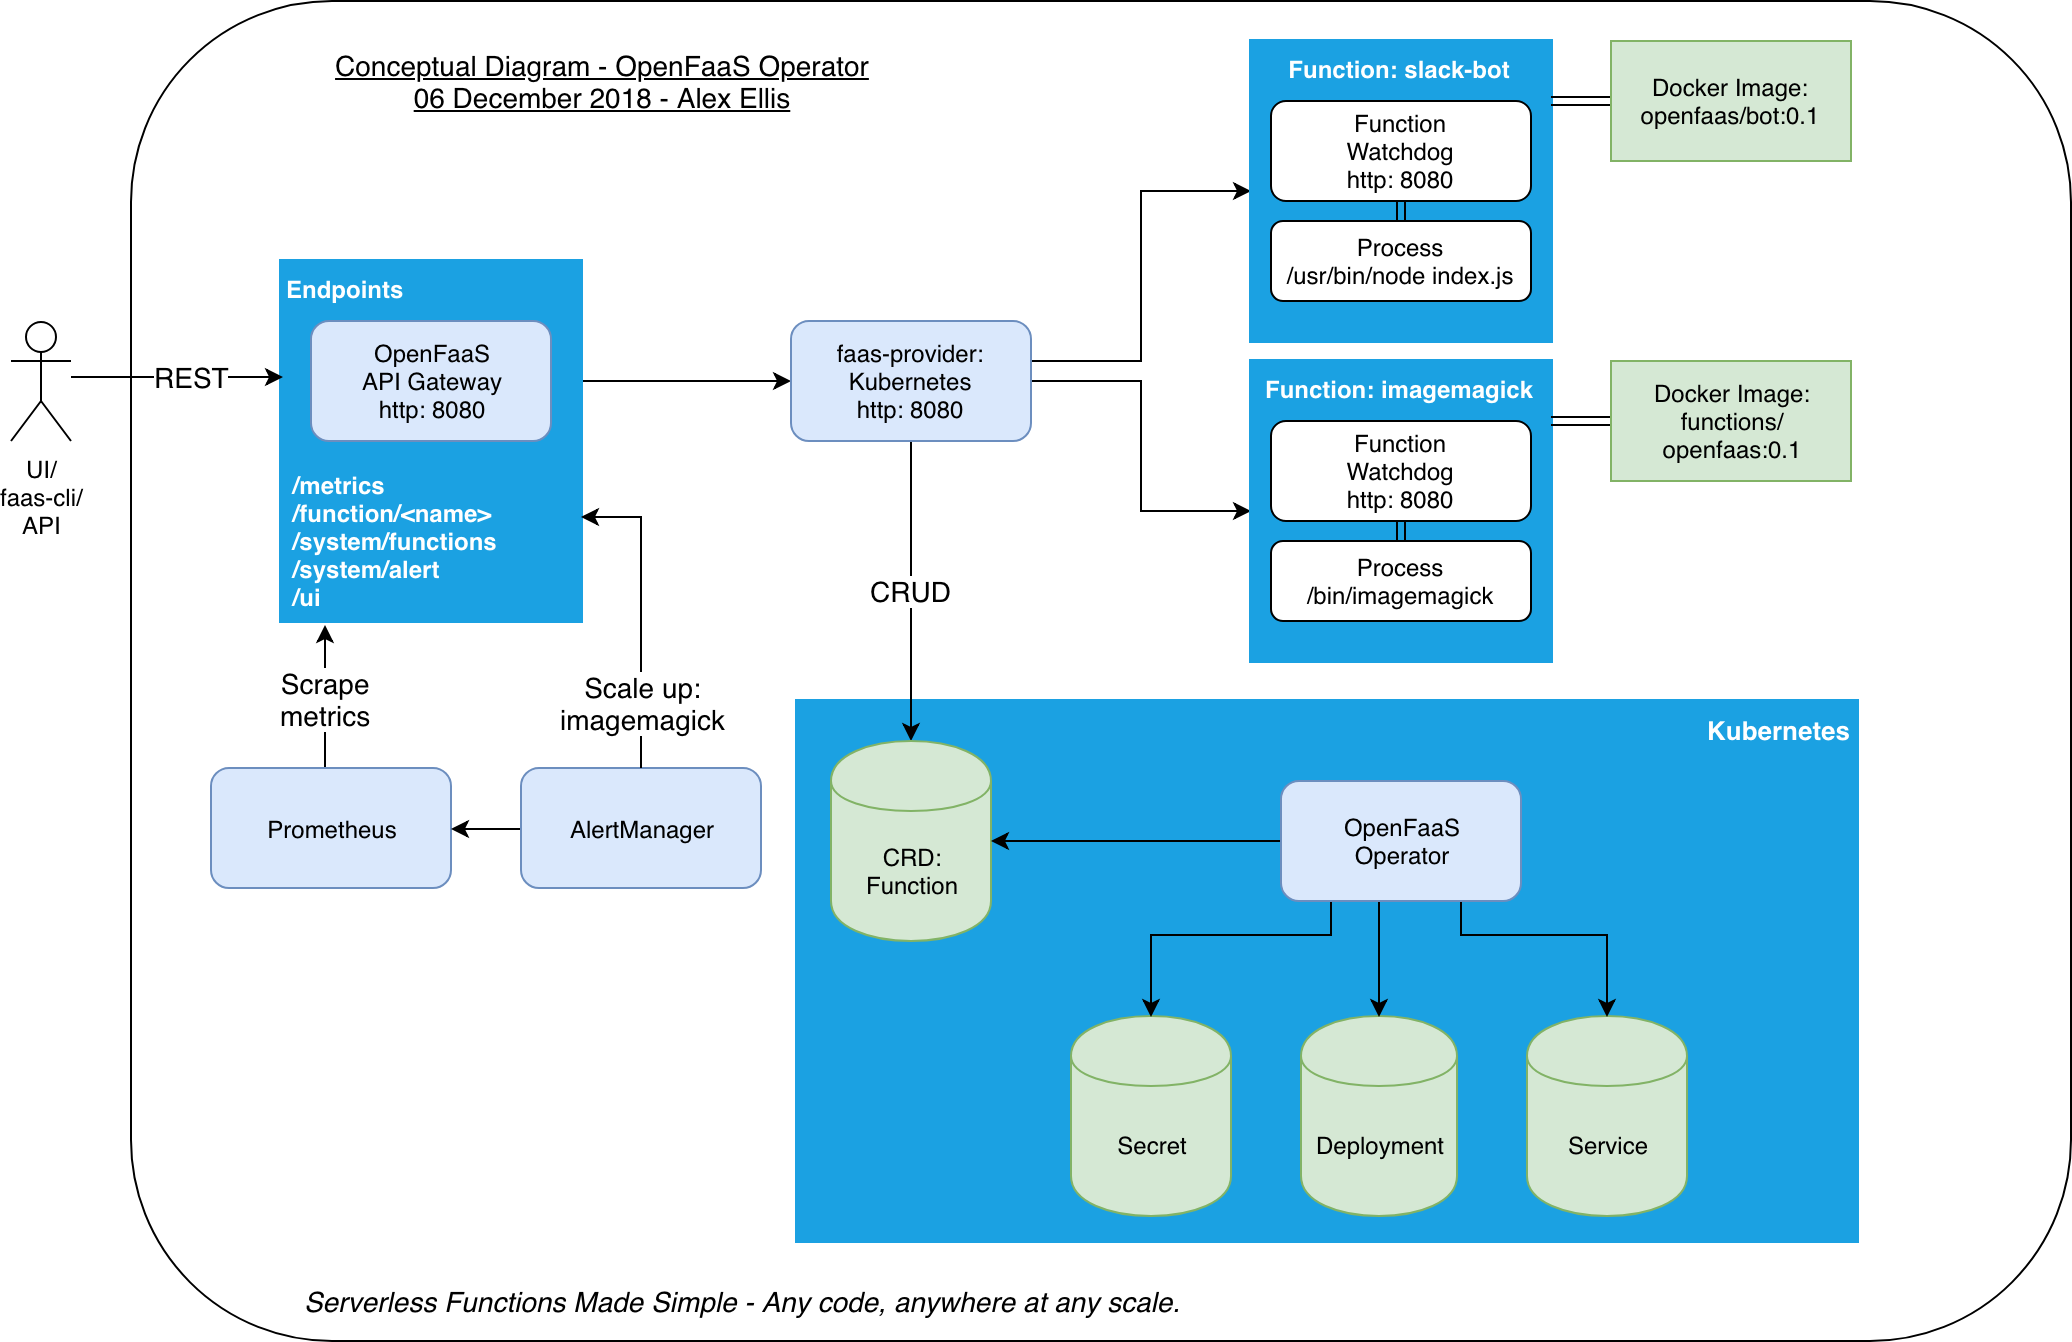
\includegraphics[width=14cm]{graphics/diagrams/openfaas-gateway-architecture.png}
    \caption{Diagram showing the architecture and components of OpenFaaS, in particular the OpenFaaS API Gateway. Taken from the official OpenFaaS architecture documentation\cite{openfaas-gateway}}
    \label{fig:openfaas-gateway-diagram}
\end{figure}


As mentioned in the background chapter, OpenFaaS uses Linux containers to run functions, and in turn Kubernetes to manage these containers. To clarify the role our load balancer would take in a serverless system, we describe how it would affect OpenFaaS. By default OpenFaaS employs a component they call \textit{API Gateway}. This API Gateway is the component which first receives \textbf{all} client requests, and then continues to send them on to the corresponding functions, while at the same time collecting metrics used by the system for tasks like auto-scaling. Figure \ref{fig:openfaas-gateway-diagram}, which is taken directly from the official OpenFaaS documentation shows the interactions with the other components of the system. Since the API Gateway is just another container running in Kubernetes\cite{kubernetes}, and failover capability is a concern, there can be multiple instances of the API Gateway running at any given time.
As discussed a major reason for the sub-optimal performance of network bound workloads in edge scenarios is the lack of efficient request routing.
In the case of OpenFaaS this stems from it delegating networking and routing tasks to Kubernetes, since it is the underlying container orchestration platform. This applies to both the initial ingress into the cluster, as well as to how the API Gateway forwards client requests to the relevant replicas to be processed. Kube-proxy, the component of Kubernetes which handles networking and routing tasks, will default to the round-robin policy of selecting upstreams. While it is possible to set up kube-proxy in a way that will prefer nodes in the same zone based on a label, this functionality is built around cloud based deployments and is insufficient to address the heterogeneity in networking and compute power introduced by edge computing. This defaulting to round-robin means that in effect, serverless frameworks such as OpenFaaS route the requests basically at random between the entry point in the network and the API Gateway, and then from the API Gateway to the relevant function.\\
In our approach the load balancer takes the role the API Gateway has in OpenFaaS. It is characterized by being
\begin{enumerate}
    \item the entry point for the client to the serverless system, meaning there are no network hops between the load balancer instance and the node the request originally arrived at, and
    \item directly forwarding requests to the corresponding serverless function instances.
\end{enumerate}
When implementing our proposed approach in practise this would mean that the serverless framework would have to be adapted to fulfill these conditions for the load balancer. If these conditions aren't met, this would likely negate the positive affect our approach has on performance.

As an example in the case of OpenFaaS, referencing the OpenFaaS architecture in Figure \ref{fig:openfaas-gateway-diagram}, this could be realized in the following ways:
\begin{enumerate}
    \item API Gateways and load balancers are scaled and scheduled together, meaning they are always co-located on the same node. The API-Gateway would then still first receive requests and handle implementation specific tasks for the serverless system, but then forward the request to the load balancer instance on the same node, which then decides on further request routing.
    \item The load balancer is the new entry point for clients, effectively replacing the API Gateway. In this scenario the load balancer and API Gateway would also be altered such that metrics and information relevant to the system could be collected by the load balancers and forwarded to API Gateway instances, which then handle them as before.
\end{enumerate}

\subsection{Load Balancing Concepts}

% Target: 8 pages with figures
\section{Scaling and Scheduling}

\chapter{Evaluation}
% about 18 pages, split between text and figures
\chapter{Results}
% target: 9ish pages
\chapter{Discussion}
% \chapter{Introduction}
% \todo{Enter your text here.}

% \chapter{Additional Chapter}
% \todo{Enter your text here.}

% Remove following line for the final thesis.
% %% intro.tex
%% Copyright (C) 2014-2020 by Thomas Auzinger <thomas@auzinger.name>
%
% This work may be distributed and/or modified under the
% conditions of the LaTeX Project Public License, either version 1.3
% of this license or (at your option) any later version.
% The latest version of this license is in
%   http://www.latex-project.org/lppl.txt
% and version 1.3 or later is part of all distributions of LaTeX
% version 2005/12/01 or later.
%
% This work has the LPPL maintenance status `maintained'.
%
% The Current Maintainer of this work is Thomas Auzinger.
%
% This work consists of the files vutinfth.dtx and vutinfth.ins
% and the derived file vutinfth.cls.
% This work also consists of the file intro.tex.


\newacronym{ctan}{CTAN}{Comprehensive TeX Archive Network}
\newacronym{faq}{FAQ}{Frequently Asked Questions}
\newacronym{pdf}{PDF}{Portable Document Format}
\newacronym{svn}{SVN}{Subversion}
\newacronym{wysiwyg}{WYSIWYG}{What You See Is What You Get}

\newglossaryentry{texteditor}
{
  name={editor},
  description={A text editor is a type of program used for editing plain text files.}
}

\chapter{Introduction to \LaTeX}

Since \LaTeX\ is widely used in academia and industry, there exists a plethora of freely accessible introductions to the language.
Reading through the guide at \url{https://en.wikibooks.org/wiki/LaTeX} serves as a comprehensive overview for most of the functionality and is highly recommended before starting with a thesis in \LaTeX.

\section{Installation}

A full \LaTeX\ distribution\index{distribution} consists not only of the binaries that convert the source files to the typeset documents, but also of a wide range of packages and their documentation.
Depending on the operating system, different implementations are available as shown in Table~\ref{tab:distrib}.
\textbf{Due to the large amount of packages that are in everyday use and due to their high interdependence, it is paramount to keep the installed distribution\index{distribution} up to date.}
Otherwise, obscure errors and tedious debugging ensue.

\begin{table}
  \centering
  \begin{tabular}{cccc}
    \toprule
    Distribution & Unix         & Windows      & MacOS        \\
    \midrule
    TeX Live     & \textbf{yes} & yes          & (yes)        \\
    MacTeX       & no           & no           & \textbf{yes} \\
    MikTeX       & (yes)        & \textbf{yes} & yes          \\
    \bottomrule
  \end{tabular}
  \caption{\TeX/\LaTeX\ distributions for different operating systems. Recomended choice in \textbf{bold}.}
  \label{tab:distrib} % \label has to be placed AFTER \caption to produce correct cross-references.
\end{table}

\section{Editors}

A multitude of \TeX\ \glspl{texteditor} are available differing in their editing models, their supported operating systems and their feature sets.
A comprehensive overview of \glspl{texteditor} can be found at the Wikipedia page  \url{https://en.wikipedia.org/wiki/Comparison_of_TeX_editors}.
TeXstudio (\url{http://texstudio.sourceforge.net/}) is recommended.
Most editors support a synchronization of the generated document and the \LaTeX\ source by \verb|Ctrl| clicking either on the source document or the generated document.

\section{Compilation}

Modern editors usually provide the compilation programs to generate \gls{pdf} documents and for most \LaTeX\ source files, this is sufficient.
More advanced \LaTeX\ functionality, such as glossaries and bibliographies, needs additional compilation steps, however.
It is also possible that errors in the compilation process invalidate intermediate files and force subsequent compilation runs to fail.
It is advisable to delete intermediate files (\verb|.aux|, \verb|.bbl|, etc.), if errors occur and persist.
All files that are not generated by the user are automatically regenerated.
To compile the current document, the steps as shown in Table~\ref{tab:compile} have to be taken.


\begin{table}
  \centering
  \begin{tabular}{rl}
    \toprule
    & Description \\
    \midrule
    1 & Scan for refs, toc/lof/lot/loa items and cites \\
    2 & Build the bibliography     \\
    3 & Link refs and build the toc/lof/lot/loa \\
    4 & Link the bibliography \\
    5 & Build the glossary \\
    6 & Build the acronyms \\
    7 & Build the index \\
    8 & Link the glossary, acronyms, and the index \\
    9 & Link the bookmarks \\
    \midrule
    & Command \\
    \midrule
    1 & \verb|pdflatex.exe  example| \\
    2 & \verb|bibtex.exe    example| \\
    3 & \verb|pdflatex.exe  example| \\
    4 & \verb|pdflatex.exe  example| \\
    5 & \verb|makeindex.exe -t example.glg -s example.ist| \\
      & \verb|              -o example.gls example.glo| \\
    6 & \verb|makeindex.exe -t example.alg -s example.ist| \\
      & \verb|              -o example.acr example.acn| \\
    7 & \verb|makeindex.exe -t example.ilg -o example.ind example.idx| \\
    8 & \verb|pdflatex.exe  example| \\
    9 & \verb|pdflatex.exe  example| \\
    \bottomrule
  \end{tabular}
  \caption{Compilation steps for this document. The following abbreviations were used: table of contents (toc), list of figures (lof), list of tables (lot), list of algorithms (loa).}
  \label{tab:compile} % \label has to be placed AFTER \caption to produce correct cross-references.
\end{table}


\section{Basic Functionality}

In this section, various examples are given of the fundamental building blocks used in a thesis.
Many \LaTeX\ commands have a rich set of options that can be supplied as optional arguments.
The documentation of each command should be consulted to get an impression of the full spectrum of its functionality.

\subsection{Floats}

Two main categories of page elements can be differentiated in the usual \LaTeX\ workflow: \textit{(i)} the main stream of text and \textit{(ii)} floating containers that are positioned at convenient positions throughout the document.
In most cases, tables, plots, and images are put into such containers since they are usually positioned at the top or bottom of pages.
These are realized by the two environments \verb|figure| and \verb|table|, which also provide functionality for cross-referencing (see Table~\ref{tab:intro} and Figure~\ref{fig:intro}) and the generation of corresponding entries in the list of figures and the list of tables.
Note that these environments solely act as containers and can be assigned arbitrary content.

\subsection{Tables}

A table in \LaTeX\ is created by using a \verb|tabular| environment or any of its extensions, e.g., \verb|tabularx|.
The commands \verb|\multirow| and \verb|\multicolumn| allow table elements to span multiple rows and columns.

\begin{table}[h] % placement specifier
  \centering
  \begin{tabular}{lll}
    \toprule
    \multicolumn{2}{c}{Position} \\
    \cmidrule{1-2} % partial horizontal rule
    Group & Abbrev & Name \\
    \midrule
    Goalkeeper & GK & Paul Robinson \\
    \midrule
    \multirow{4}{*}{Defenders} & LB & Lucus Radebe \\
                               & DC & Michael Duburry \\
                               & DC & Dominic Matteo \\
                               & RB & Didier Domi \\
    \midrule
    \multirow{3}{*}{Midfielders} & MC & David Batty \\
                                 & MC & Eirik Bakke \\
                                 & MC & Jody Morris \\
    \midrule
    Forward & FW & Jamie McMaster \\
    \midrule
    \multirow{2}{*}{Strikers} & ST & Alan Smith \\
                              & ST & Mark Viduka \\
    \bottomrule
  \end{tabular}
  \caption{Adapted example from the \LaTeX guide at \url{https://en.wikibooks.org/wiki/LaTeX/Tables}. This example uses rules specific to the \texttt{booktabs} package and employs the multi-row functionality of the \texttt{multirow} package.}
  \label{tab:intro} % \label has to be placed AFTER \caption to produce correct cross-references.
\end{table}

\subsection{Images}

An image is added to a document via the \verb|\includegraphics| command as shown in Figure~\ref{fig:intro}.
The \verb|\subcaption| command can be used to reference subfigures, such as Figure~\ref{fig:intro:full width} and~\ref{fig:intro:half width}.

\begin{figure}[h]
  \centering
  \begin{subfigure}[b]{0.45\columnwidth}
    \centering
    
\includegraphics[width=\textwidth]{Logo-schwarz.pdf}
    \subcaption{The header logo at text width.}
    \label{fig:intro:full width}
  \end{subfigure}
  \begin{subfigure}[b]{0.45\columnwidth}
    \centering
    
\includegraphics[width=0.5\textwidth]{Logo-schwarz.pdf}
    \subcaption{The header logo at half the text width.}
    \label{fig:intro:half width}
  \end{subfigure}
  \caption[Optional caption for the figure list (often used to abbreviate long captions)]{The header logo at different sizes.} % Remove the [...] argument if the original caption should be used in the figure list.
  \label{fig:intro} % \label has to be placed AFTER \caption (or \subcaption) to produce correct cross-references.
\end{figure}

\subsection{Mathematical Expressions}

One of the original motivation to create the \TeX\ system was the need for mathematical typesetting.
To this day, \LaTeX\ is the preferred system to write math-heavy documents and a wide variety of functions aids the author in this task.
A mathematical expression can be inserted inline as $\sum_{n=1}^{\infty} \frac{1}{n^2} = \frac{\pi^2}{6}$ outside of the text stream as \[ \sum_{n=1}^{\infty} \frac{1}{n^2} = \frac{\pi^2}{6} \] or as numbered equation with
\begin{equation}
\sum_{n=1}^{\infty} \frac{1}{n^2} = \frac{\pi^2}{6}.
\end{equation}

\subsection{Pseudo Code}

The presentation of algorithms can be achieved with various packages; the most popular are \verb|algorithmic|, \verb|algorithm2e|, \verb|algorithmicx|, or \verb|algpseudocode|.
An overview is given at \url{https://tex.stackexchange.com/questions/229355}.
An example of the use of the \verb|alogrithm2e| package is given with Algorithm~\ref{alg:gauss-seidel}.

\begin{algorithm}
  \SetKw{BreakFor}{break for}
  \KwIn{A scalar~$\epsilon$, a matrix $\mathbf{A} = (a_{ij})$, a vector $\vec{b}$, and an initial vector $\vec{x}^{(0)}$}
  \KwOut{$\vec{x}^{(n)}$ with $\mathbf{A} \vec{x}^{(n)} \approx \vec{b}$}
  \For{$k\leftarrow 1$ \KwTo maximum iterations}
  {
     \For{$i\leftarrow 1$ \KwTo $n$}
     {
        $x_i^{(k)} = \frac{1}{a_{ii}} \left(b_i-\sum_{j<i} a_{ij} x_j^{(k)} - \sum_{j>i} a_{ij} x_j^{(k-1)} \right)$\;
     }
     \If{$\lvert\vec{x}^{(k)}-\vec{x}^{(k-1)}\rvert < \epsilon$}
     {\BreakFor\;}
  }
  \Return{$\vec{x}^{(k)}$\;}
  \caption{Gauss-Seidel}
  \label{alg:gauss-seidel} % \label has to be placed AFTER \caption to produce correct cross-references.
\end{algorithm}

\section{Bibliography}

The referencing of prior work is a fundamental requirement of academic writing and well supported by \LaTeX.
The \textsc{Bib}\TeX\ reference management software is the most commonly used system for this purpose.
Using the \verb|\cite| command, it is possible to reference entries in a \verb|.bib| file out of the text stream, e.g., as~\cite{Turing1936}.
The generation of the formatted bibliography needs a separate execution of \verb|bibtex.exe| (see Table~\ref{tab:compile}).

\section{Table of Contents}

The table of contents is automatically built by successive runs of the compilation, e.g., of \verb|pdflatex.exe|.
The command \verb|\setsecnumdepth| allows the specification of the depth of the table of contents and additional entries can be added to the table of contents using \verb|\addcontentsline|.
The starred versions of the sectioning commands, i.e., \verb|\chapter*|, \verb|\section*|, etc., remove the corresponding entry from the table of contents.

\section{Acronyms / Glossary / Index}

The list of acronyms, the glossary, and the index need to be built with a separate execution of \verb|makeindex| (see Table~\ref{tab:compile}).
Acronyms have to be specified with \verb|\newacronym| while glossary entries use \verb|\newglossaryentry|.
Both are then used in the document content with one of the variants of \verb|\gls|, such as \verb|\Gls|, \verb|\glspl|, or \verb|\Glspl|.
Index items are simply generated by placing \verb|\index|\marg{entry} next to all the words that correspond to the index entry \meta{entry}.
Note that many enhancements exist for these functionalities and the documentation of the \verb|makeindex| and the \verb|glossaries| packages should be consulted.

\section{Tips}

Since \TeX\ and its successors do not employ a \gls{wysiwyg} editing scheme, several guidelines improve the readability of the source content:
\begin{itemize}
\item Each sentence in the source text should start with a new line.
      This helps not only the user navigation through the text, but also enables revision control systems (e.g. \gls{svn}, Git) to show the exact changes authored by different users.
      Paragraphs are separated by one (or more) empty lines.
\item Environments, which are defined by a matching pair of \verb|\begin{name}| and \verb|\end{name}|, can be indented by whitespace to show their hierarchical structure.
\item In most cases, the explicit use of whitespace (e.g. by adding \verb|\hspace{4em}| or \verb|\vspace{1.5cm}|) violates typographic guidelines and rules.
      Explicit formatting should only be employed as a last resort and, most likely, better ways to achieve the desired layout can be found by a quick web search.
\item The use of bold or italic text is generally not supported by typographic considerations and the semantically meaningful \verb|\emph{|\texttt{$\dots$}\verb|}| should be used.
\end{itemize}

The predominant application of the \LaTeX\ system is the generation of \gls{pdf} files via the \textsc{Pdf}\LaTeX\ binaries.
In the current version of \textsc{Pdf}\LaTeX, it is possible that absolute file paths and user account names are embedded in the final \gls{pdf} document.
While this poses only a minor security issue for all documents, it is highly problematic for double blind reviews.
The process shown in Table~\ref{tab:ps2pdf} can be employed to strip all private information from the final \gls{pdf} document.

\begin{table}[h]
  \centering
  \begin{tabular}{rl}
  \toprule
  & Command \\
  \midrule
  1 & Rename the \gls{pdf} document \verb|final.pdf| to \verb|final.ps|. \\
  2 & Execute the following command: \\
    & \verb|ps2pdf -dPDFSETTINGS#/prepress ^| \\
    & \verb| -dCompatibilityLevel#1.4 ^| \\
    & \verb| -dAutoFilterColorImages#false ^| \\
    & \verb| -dAutoFilterGrayImages#false ^| \\
    & \verb| -dColorImageFilter#/FlateEncode ^| \\
    & \verb| -dGrayImageFilter#/FlateEncode ^| \\
    & \verb| -dMonoImageFilter#/FlateEncode ^| \\
    & \verb| -dDownsampleColorImages#false ^| \\
    & \verb| -dDownsampleGrayImages#false ^| \\
    & \verb| final.ps final.pdf| \\
  \bottomrule
  \end{tabular}

  On Unix-based systems, replace \verb|#| with \verb|=| and \verb|^| with \verb|\|.
  \caption{Anonymization of \gls{pdf} documents.}
  \label{tab:ps2pdf}
\end{table}

\section{Resources}

\subsection{Useful Links}

In the following, a listing of useful web resources is given.
\begin{description}
\item[\url{https://en.wikibooks.org/wiki/LaTeX}] An extensive wiki-based guide to \LaTeX.
\item[\url{http://www.tex.ac.uk/faq}] A (huge) set of \gls{faq} about \TeX\ and \LaTeX.
\item[\url{https://tex.stackexchange.com/}] The definitive user forum for non-trivial \LaTeX-related questions and answers.
\end{description}

\subsection[Comprehensive TeX Archive Network]{\gls{ctan}}

The \gls{ctan} is the official repository for all \TeX\ related material.
It can be accessed via \url{https://www.ctan.org/} and hosts (among other things) a huge variety of packages that provide extended functionality for \TeX\ and its successors.
Note that most packages contain \gls{pdf} documentation that can be directly accessed via \gls{ctan}.

In the following, a short, non-exhaustive list of relevant \gls{ctan}-hosted packages is given together with their relative path.
\begin{description}[itemsep=0ex]
\item[\href{https://www.ctan.org/pkg/algorithm2e}{algorithm2e}] Functionality for writing pseudo code.
\item[\href{https://www.ctan.org/pkg/amsmath}{amsmath}] Enhanced functionality for typesetting mathematical expressions.
\item[\href{https://www.ctan.org/pkg/amsfonts}{amssymb}] Provides a multitude of mathematical symbols.
\item[\href{https://www.ctan.org/pkg/booktabs}{booktabs}] Improved typesetting of tables.
\item[\href{https://www.ctan.org/pkg/enumitem}{enumitem}] Control over the layout of lists (\verb|itemize|, \verb|enumerate|, \verb|description|).
\item[\href{https://www.ctan.org/pkg/fontenc}{fontenc}] Determines font encoding of the output.
\item[\href{https://www.ctan.org/pkg/glossaries}{glossaries}] Create glossaries and list of acronyms.
\item[\href{https://www.ctan.org/pkg/graphicx}{graphicx}] Insert images into the document.
\item[\href{https://www.ctan.org/pkg/inputenc}{inputenc}] Determines encoding of the input.
\item[\href{https://www.ctan.org/pkg/l2tabu}{l2tabu}] A description of bad practices when using \LaTeX.
\item[\href{https://www.ctan.org/pkg/mathtools}{mathtools}] Further extension of mathematical typesetting.
\item[\href{https://www.ctan.org/pkg/memoir}{memoir}] The document class on upon which the \verb|vutinfth| document class is based.
\item[\href{https://www.ctan.org/pkg/multirow}{multirow}] Allows table elements to span several rows.
\item[\href{https://www.ctan.org/pkg/pgfplots}{pgfplots}] Function plot drawings.
\item[\href{https://www.ctan.org/pkg/pgf}{pgf/TikZ}] Creating graphics inside \LaTeX\ documents.
\item[\href{https://www.ctan.org/pkg/subcaption}{subcaption}] Allows the use of subfigures and enables their referencing.
\item[\href{https://www.ctan.org/tex-archive/info/symbols/comprehensive/}{symbols/comprehensive}] A listing of around 5000 symbols that can be used with \LaTeX.
\item[\href{https://www.ctan.org/pkg/voss-mathmode}{voss-mathmode}] A comprehensive overview of typesetting mathematics in \LaTeX.
\item[\href{https://www.ctan.org/pkg/xcolor}{xcolor}] Allows the definition and use of colors.
\end{description} % A short introduction to LaTeX.

\backmatter

% Use an optional list of figures.
\listoffigures % Starred version, i.e., \listoffigures*, removes the toc entry.

% Use an optional list of tables.
\cleardoublepage % Start list of tables on the next empty right hand page.
\listoftables % Starred version, i.e., \listoftables*, removes the toc entry.

% Use an optional list of alogrithms.
\listofalgorithms
\addcontentsline{toc}{chapter}{List of Algorithms}

% Add an index.
\printindex

% Add a glossary.
\printglossaries

% Add a bibliography.
\bibliographystyle{alphaurl}
\bibliography{main}

\end{document}